\documentclass[5p]{elsarticle}
\usepackage{graphicx}
\graphicspath{ {pic/} }
\usepackage{lineno,hyperref}
\usepackage{amsmath}
\usepackage{natbib}

%https://www.cnblogs.com/coolqiyu/p/5580290.html
\usepackage[noend]{algpseudocode}
\usepackage{algorithmicx,algorithm}
\modulolinenumbers[5]

\journal{DPDC}

\bibliographystyle{elsarticle-num}
%%%%%%%%%%%%%%%%%%%%%%%
\newcommand{\dabiaolv}{reach rate}


\begin{document}

\begin{frontmatter}

\title{A data-driven approach for performance evaluation for cache groups in content delivery network
    %\tnoteref{mytitlenote}
    %JPDC-A data-driven framework for performance evaluation for CDN cache groups
    }
%\tnotetext[mytitlenote]{Fully documented templates are available in the elsarticle package on %\href{http://www.ctan.org/tex-archive/macros/latex/contrib/elsarticle}{CTAN}.}

%% Group authors per affiliation:
\author{None
    %\fnref{myfootnote}
    }
\address{Radarweg 29, Amsterdam}
%\fntext[myfootnote]{Since 1880.}

%% or include affiliations in footnotes:
\author[mymainaddress,mysecondaryaddress]{Elsevier Inc}
\ead[url]{www.elsevier.com}

\author[mysecondaryaddress]{Global Customer Service\corref{mycorrespondingauthor}}
\cortext[mycorrespondingauthor]{Corresponding author}
\ead{support@elsevier.com}

\address[mymainaddress]{1600 John F Kennedy Boulevard, Philadelphia}
\address[mysecondaryaddress]{360 Park Avenue South, New York}

\begin{abstract}
CDN Service providers are increasingly using data-driven mechanisms to build their performance model of their service-providing systems. To build a model to accurately describe the performance of the existing infrastructure is very crucial to make resource management decisions. Conventional approaches that use hand-tuned parameters has its drawback. Recently, data-driven paradigm have been shown to greatly outperform traditional methods in many applications, in both accuracy and their quick reactions to the changing environment. We design a framework that using these techniques to build a performance model. Our approach shows an average 6.98\% improvement in terms of weighted mean absolute percent error (WMAPE) compared to the baseline models.
\end{abstract}
\begin{keyword}
\textit{edge computing, deep learning, content delivery networks, sequence learning, predictive analysis, high dimensional data}
%\texttt{elsarticle.cls}\sep \LaTeX\sep Elsevier \sep template
%\MSC[2010] 00-01\sep  99-00
\end{keyword}
\end{frontmatter}
\linenumbers
\section{Introduction}
% the detail of absract
There is a trend \cite{Jiang2017Pytheas:Exploration-Exploitation} \cite{Mao2017NeuralPensieve} that using data-driven methods to model complex networked systems. Traditional approach typically simple huristics. These methods have several drawbacks.They cannot accurately reflect and oversimplified the complex systems due to the lack of knowledge of real-word environment. Driven by the opportunity to collect and analyze data (e.g., application quality measurement from end users), many recent proposals have demonstrated the promise of using deep learning to characterize and optimize networked systems. Drawing parralel from the success of deep-learning on pattern recognizaition, instead of using empirical non-linear learning model to descirbe the complex interaction of different features, we use deep learning models and treat networked systems as a black-box.

A content delivery network (CDN) is a globally distributed network system deployed across the Internet. Composed with geographically distributed cache servers, CDNs deliver cached content  to  customers  worldwide  based  on their geographic locations. Extensively  using  cache  servers,  content  delivery over  CDN  has  low  latency  and  high  reliability,  and  supports better quality of experience.

The CDN Service providers are increasingly using data-driven mechanisms to build their performance model of their service-providing systems. To build a model to accurately provice an understanding of the performance of the existing infrastructure such as the health of cache groups and network status, is very crucial to make resource management decisions including content placement, network traffic scheduling, load banlance of the CDN network. Modeling all available physical resources, we can maximize a resource utilization in terms of service quality, cost, profit, etc.

Generally CDN provicers don't have direct measurement from the clients (the logs from video players, web browser that can show the QoE of clients). Instead, they use the indirect measurement \dabiaolv defined in Section II which is collected and analyzed from the log of the HA proxy of CDN cache groups, which is . The computation of \dabiaolv is done offline. In order to enable themselves make resource manangement decisions in real time, the CDN providers have to use the metrics that can be collected in the real time to infer the \dabiaolv. 

Cache group can be characterised as multi-dimensional, highly non-linear, time variant vecrors. The metrics that collected from members of the CDN cache groups are sequence data that are measured every minute, which have hundreds of dimensions. The state-of-art methods are typically using simple huristics, which are over-simplifed and baised due to the human experience. 

%Resouoce management involves 
We frame our problem as a sequence learning problem, which consists of stages: (1) feature engineering (2) representaion learning by lstm auto-encoder (3) fully connected network/ svm/ other black-box machine learning algorithm to output the predictions. 
%\deep-
lstm,lstm auto encoder and decoder

Our main contributions are listed below:
\begin{itemize}
  \item data-driven approach
  \item performance modeling as sequence modeling problem
  \item anomaly detection(Collective Anomalies a) and prediction
\end{itemize}

The remain organization of this paper is as follows. In Section II, we first  introduce the formulation of performance evaluation problem and  then introduce  our LSTM  based  structure. In Section III, we introduce reach-rate prediction algorithms based on the
auto-encoder and decoder. In Section IV, we demonstrate performance  improvements over baseline models. Finally, we provide concluding remarks in Section V.
%\cite
\section{Background}
\begin{figure}[h]
    \centering
    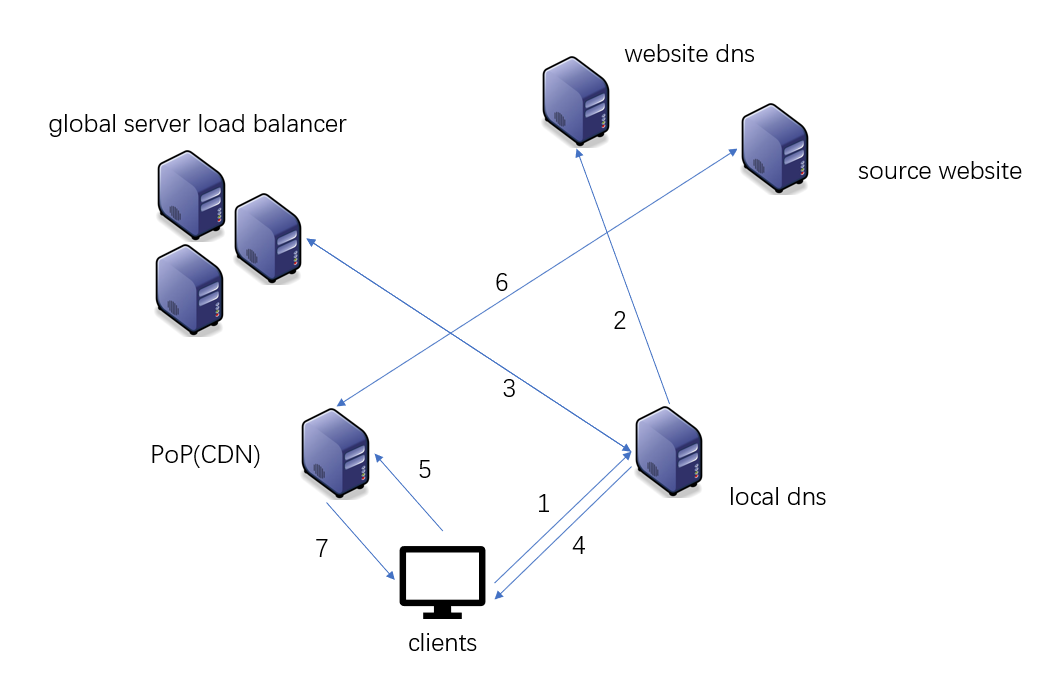
\includegraphics[width=0.5\textwidth]{CDN_new.png}
    \caption{The architecture of CDN}
    \label{fig}
\end{figure}

\begin{figure}[h]
    \centering
    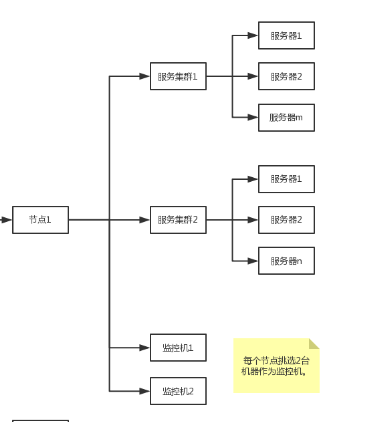
\includegraphics[width=0.5\textwidth]{cache_group.png}
    \caption{The figure}
    \label{fig: the structure of PoP}
\end{figure}

A content delivery network or content distribution network (CDN) (figure 1) is a geographically distributed network of cache servers. CDN helps content provider deliver web pages and other multi-media content to the clients, based on the locations of the clients and cache servers nearby the clients. The basic working procedure is as follows. Step 1:client send a request to local dns. Step 2: the DNS finds the CNAME and redirects the request to the gslb (global sever load balance). Step 3: the local DNS server sends request to the glsb and glsb returns the ip address of CDN servers based on the scheduling policy. Step 4: the local DNS return the ip address to the clients. Step 5: fetch


A CDN cache server group is the basic resource scheduling unit for CDN. A CDN cache group is a load banlanced cluster that consists of interconnetcted cache servers. A typical implementation consists of HAPROXY and squid servers. The requests from clients are distributed by HAproxy to cache servers. HAproxy use be set to use different algorithms algorithms to maximize the utilization of every server. Round-robin algorithm distributes the load equally to each server. In heterogeneous cluster,  weighted round-robin algorithm is used. A weight was assigned to the server based on its processing capabilities. A heterogeneous strucutre of a cluster adds comlexity to the feature enginnring, as we will discuss later.

As CDN providers don't have direct QoS measurement from the clients (the logs from video players, web browser that can show the QoE), so they use the indirect measurement \dabiaolv which is collected from log of the HA proxy of CDN cache groups. 
根据haproxy的日志计算标签数据,即达标率。
达标率的计算公式为:响应速度=内核响应发送长度/响应完整发送时间;
达标:响应速度>达标率配置速度阈值 则达标;
响应日志记录数=一分钟内总请求数
达标率 =达标数/总请求数

The data we collected are listed in table. We collected about 130 metrics. It can rouphlyy grouped in the following broad categories: CPU utilization. Network utilization. disk utilization. memory utilization.
\section{Problem formulation and Model}


we argue that performance evlaluation as a sequence learning problem. Since we are able to collect the caching servers performance metrics and network metrics at a certain time interval, we can use a sequence models to describe relationship between metrics from  cache groups and \dabiaolv

There are four catogories of sequence learning problem, which are many to one, many to one and many one. Our goal is to model the relationship between collected metrics and \dabiaolv. In general, we can use the following formulation to describe the prediction process.

\begin{figure}[h]
    \centering
    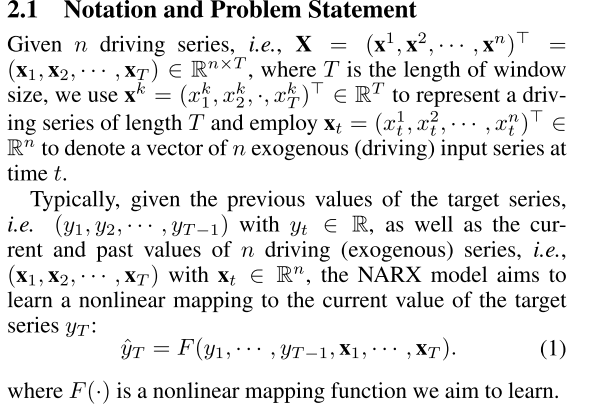
\includegraphics[width=0.5\textwidth]{notation_and_problem_statement.png}
    \caption{}
    \label{fig:notation_and_problem_statement}
\end{figure}

The training phase is to learn a best function that minimizes the prediction error as follows:
\begin{equation}
	%\mathbf h_t = \tanh(\mathbf W * \mathbf h_{t-1} + \mathbf I * \x_t)
\end{equation}

Many models can be used to approximate f in sequence modeling. Conventional approaches use AR models. The AR method builds a model of the time series that is composed of a linear part and a random noise part. Whilst the linear part models the ascertainable chunk of the time series, the random noise reflects the unpredictable randomness in the time series. Furthermore, the linear part incorporates historical values of the time series, which also form the order of the AR model. One commonly refers to the notation AR(l) to indicate how much historical information is used to build the AR model. Equation shows the general autoregressive model for the univariate case. Here, y denotes the time series to be modelled, c denotes the constant parameter of the linear decomposition, β denotes the model to be computed and epsilon reflects the random noise part.

\begin{align}
    y_t = c+\sum_{i=1}^{l}(\beta_i ∗ y_t_−_i)+\epsilon_t
\end{align}


VAR model is a generalization fo AR models. In VAR models, the relationship between the predictor and the target variable is simply described using a linear model as follows: It is used to find a linear model that incorporates the influence of multiple time series into the actual value of a target variable yt.

As such, the equation contains the vectors Yt, Yt−l, the values ?t, c and the model matrices Al. The vectors Yt and Yt−l are composed of all incorporated variables (x, y, z, ...) at time stamp t and t − l. Hence, the i-th element in these vectors is the i-th incorporated variable at the respective time stamps. The matrices A1 . . .Al
reflect the models that need to be fitted. The VAR model is shown in equation 2.21.

\begin{align}
    equation of VAR
\end{align}

Linear models are easy to implement and have good interpretation and thus are widely used in many real work time series analysis problems. However, linear models are shown not sufficient to describe some nonlinear behaviors of the complex network systems. In many cases, neural networks tend to outperform AR-based models [A comparison of artificial neural network and time series models for forecasting commodity prices]. We use deep learning as alternaives.

Deep learning (DL) is a branch of machine learning based on a set of algorithms that attempts to model high-level abstractions in data by using artificial neural network (ANN) ()Figure) architectures composed of multiple non-linear transformations. They have a lot of successful applications in speech and image recognition, machine translation, and forecasting of financial time series. Compared to other machine learning techniques, it can detect complex relationships among features,can extract hierarchical level of features from raw data. So it can produce more accurate result and build a model more with less time. They are advantageous for modeling intricate systems because neural networks do not require the user to predefine the feature interactions in the model, which assumes relationships within the data. Instead, the neural network searches for patterns and interactions between features to automatically generate a best fit model.

The essence of DL is to compute hierarchical features or representations of obser-vational data, where the higher-level features or factors are defined from primary lower-level measurements. Based on the features extracted from the data in the training set, the calculations within the model are adjusted so that known inputs produce desired outputs

One of the more popular DL deep neural networks is the Recurrent Neural Network (RNN). RNNs are a class of neural networks that depend on the sequential nature of their input. Such inputs could be text, speech, time series, and anything else in which the occurrence of an element in the sequence is dependent on the elements that appeared before it.

\subsection{deep learning in sequence learning}
Sequence prediction often involves forecasting the next value in a real valued sequence or outputting a class label for an input sequence.
\subsubsection{Basic feed forward neural network}
A generic three layered neural network is illustrated in Figure 2. In this study, the input matrix is an x (m x n) array where is the number of training examples and is the number of features (DC input variables), including the IT load, weather conditions, number of chillers and cooling towers running, equipment setpoints, etc. The input matrix is then multiplied by the model parameters matrix x θ 1 to produce the hidden state matrix [6]. In practice, acts as an intermediary state that interacts with the second a a parameters matrix θ 2 to calculate the output h (x)θ [6]. The size and number of hidden layers can be varied to model systems of varying complexity.

The process of training a neural network model can be broken down into four steps, each of which are covered in greater detail below: (1) Randomly initialize the model parameters , (2) Implement the forward propagation algorithm, (3) Compute the cost function J(θ) , (4) Implement the back propagation algorithm and (5) Repeat steps 2 to 4 until convergence or the desired number of iterations.

One major assumption for NNs is the independence of samples. For sequence learning problem, however, this assumption doesn't hold true, for the samples of our problem have a temporal relationship: the status of system of the next timestep not only depends on the status in the current timestep but also on the previous timesteps of indefinite length. One solution is to using a sliding window to capture the sequential relationship between the samples. The performance of this method depends on the window size, which isn't pratical for the dependencies length which isn't a fixed value. RNN eliminates the need to find the size of the window.

\subsubsection{RNN}
The promise of recurrent neural networks is that the temporal dependence and contextual
information in the input data can be learned\cite{Bengio1994LearningDifficult} \cite{ChoLearningTranslation}. 

RNNs process the input sequence one element at a time and maintain a hidden
state vector which acts as a memory for past information. They learn to selectively retain relevant information allowing them to capture dependencies across several time steps. This allows them to utilize both current input and past information while making future predictions. All this is learned by the model automatically without much knowledge of the cycles or time dependencies in data. RNNs obviate the the need for a fixed size time window and can also handle variable length sequences. Moreover, the number of states that can be represented by an NN is exponential in the number of nodes.
11

RNNs maintain a hidden vector $\mathbf h$, which is updated at time step $t$ as follows:
 
\begin{figure}[h]
    \centering
    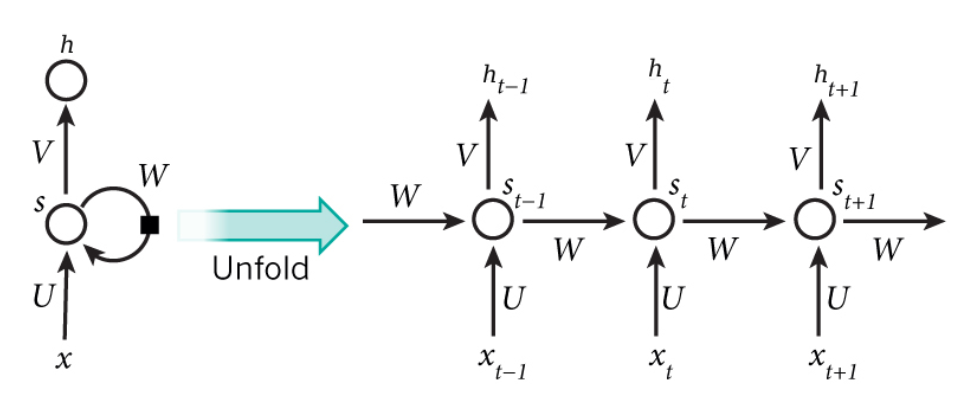
\includegraphics[width=0.5\textwidth]{RNN.png}
    \caption{RNN Architecture}
    \label{fig:RNN}
\end{figure}

\begin{equation}
	\mathbf h_t = \tanh(\mathbf W * \mathbf h_{t-1} + \mathbf I * \x_t)
\end{equation}

where $\tanh$ is the hyperbolic tangent function, $\mathbf W$ is the recurrent weight matrix and $I$ is a projection matrix. The hidden state $\mathbf h$ is then used to make a prediction

\begin{equation}
	\mathbf y_t = \text{softmax}(\mathbf W * \mathbf h_{t-1})
\end{equation}

where $\textit{softmax}$ provides a normalized probability distribution over the possible classes and $\mathbf W$ is a weight matrix. By using $\mathbf h$ as the input to another RNN, we can stack RNNs, creating deeper architectures \citep{pascanu2013construct}

\begin{equation}
	\mathbf h_t^{l} = \sigma(\mathbf W * \mathbf h_{t-1}^{l} + \mathbf I * \mathbf h_t^{l-1}).
\end{equation}

The training of RNN use back-propagation through time (BPTT). Training vanilla RNNs is known to be particularly difficult, with vanishing and exploding gradients being one possible explanation \cite{pascanu2012difficulty}. The LSTM introduced in the next section address this problems

\subsubsection{LSTM}
LSTM, introduced in \cite{Hochreiter1997LongMemory}, addresses the problem of vanishing gradients by introducing a memory cell which ensures constant error flow and gating units. \cite{MalhotraLongSeries} applied in time series. The inner working of LSTM are listed follows:
\begin{equation}
	\begin{split}
		& \mathbf g^u = \sigma(\mathbf W^u * \mathbf h_{t-1} + \mathbf I^u * \x_t) \\
		& \mathbf g^f = \sigma(\mathbf W^f * \mathbf h_{t-1} + \mathbf I^f * \x_t) \\
		& \mathbf g^o = \sigma(\macpu_usage_cpu1thbf W^o * \mathbf h_{t-1} + \mathbf I^o * \x_t) \\
		& \mathbf g^c = \tanh(\mathbf W^c * \mathbf h_{t-1} + \mathbf I^c * \x_t) \\
		& \mathbf m_t = \mathbf g^f \odot \mathbf +  \mathbf g^u \odot \mathbf g^c \\
		& \mathbf h_t = \tanh(\mathbf g^o \odot \mathbf m_{t-1})
	\end{split}
\end{equation}

\subsubsection{RNN encoder-decoder}
\cite{ChoLearningTranslation}
\begin{figure}[h]
    \centering
    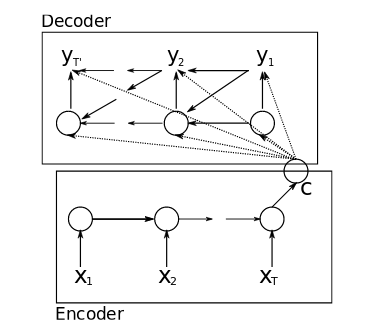
\includegraphics[width=0.5\textwidth]{RNN_encoder-decoder.png}
    \caption{neural network architecture}
    \label{fig:RNN_encoder-decoder}
\end{figure}
applications: machine translation, learning to excute, image captioning, conversational modeling

RNN Encoder-Decoder, consists of two recurrent neural networks (RNN) that act as an encoder and a decoder pair. The encoder maps a variable-length source sequence to a fixed-length vector, and the decoder maps the vector representation back to a variable-length target sequence. \cite{ChoLearningTranslation} also known as sequence embedding. The point of training an autoencoder is to make an RNN learn how to compress a relatively long sequence into a limited, dense vector.

\subsection{lstm auto-encoder}
Autoencoders are data-specific. Autoencoders are lossy. Autoencoders are learned automatically from data examples, which is a useful property: it means that it is easy to train specialized instances of the algorithm that will perform well on a specific type of input. It doesn't require any new engineering, just appropriate training data. \cite{BuildingKeras}

An autoencoder contains: an encoding function, a decoding function, and a distance function between the amount of information loss between the compressed representation of your data and the decompressed representation (i.e. a "loss" function). The encoder and decoder will be chosen to be parametric functions (typically neural networks), and to be differentiable with respect to the distance function, so the parameters of the encoding/decoding functions can be optimize to minimize the reconstruction loss, using Stochastic Gradient Descent. 


\begin{figure}[h]
    \centering
    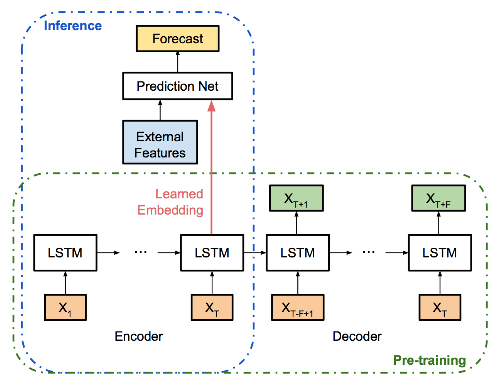
\includegraphics[width=0.5\textwidth]{neural_network_architecture.png}
    \caption{neural network architecture}
    \label{fig:neural_network_architecture}
\end{figure}


\section{Methods}
\subsection{Feature Engineering}
The feature enginnering is the process after data-clearning, in which we fill the missing data and reformating it. The propose of this stage is two-fold:

(1) to find a unified equal-length vector representation of all of the cache groups. 
The metrics collected are in the granuality of caching servers which have differnet dimensionality. As showed in graph. To make things more complex, a cache group may have dfferint number caching servers. As we only care about

(2) reduce the dimensionality for it is very time-consuming to train the models when the number of dimensionality is too high.

\subsubsection{Factors analysis}
The purpose of factors analysis is: (1) specifying the unit of analysis (2) data smurrazation data reduction (3) variable selection
As there are hundreds of variables, there are many overlaps among the variables. We use correlation in statistis to group highly correlated variables together and create composite measure that can represent each group of variables.

Correlation is an analysis of two or more observed or random variables (except in the special case of auto-correlation 2.2.1) to determine a dependence between the variables. This dependence can be classified as the probability that changes in one variable affect the behaviour of the second variable. The Pearson’s correlation , for instance, defines this dependence in the interval [−1.0, 1.0]. Pearson’s correlation for two given random variables X and Y is computed by dividing the covariance of both variables with the product of their standard deviations.

After we caculate the correlation matrix for all the features. We use DBSCAN to cluster these features to elimiate duplicated ones.

\begin{algorithm}[t]
\caption{Feature Aggregation and Selection} %算法的名字
\hspace*{0.02in} {\bf Input: list of all features listed in Table , correlation matrics} %算法的输入, \hspace*{0.02in}用来控制位置,同时利用 \\ 进行换行
\hspace*{0.02in} {\bf Output: list of all selected features} %算法的结果输出
output result
\begin{algorithmic}[1]
%\State some description % \State 后写一般语句
\For{f in F} % For 语句,需要和EndFor对应
  %\State ...
  \If{f in Cluster or labeled as noise} % If 语句,需要和EndIf对应
    \State continue
  \Else
    \State examine the Eps neighbour of f
        \if{|Eps(f)|<Minpts} then
            label f as
  \EndIf
\EndFor
\While{condition} % While语句,需要和EndWhile对应
  \State ...
\EndWhile
\State \Return result
\end{algorithmic}
\end{algorithm}

\begin{equation}
	\mathbf cor_p=p_X_,_Y = \frac{cov(X,Y)}{XY}
\end{equation}

Generally, cases of high correlation compute to a value close to 1.0, high anticorrelation is associated with a value close to -1.0 and no correlation is assumed, if the value is around 0.0. In the last case, the variables appear to be independent. Statistical correlation is used in various domains to identify and better understand relationships of variables. Examples are: medicine, biology, psychology or astronomy

Feature selection: The benefit of this feature selection process is two-fold: (a) a reduced feature set will control the model complexity during model learning, and (b) the processes gain more insights on the complex interaction of different matrics. \cite{Yeom2016Data-DrivenMatrices}. Some Deep Learning algorithms can become prohibitively computationally-expensive when dealing with high-dimensional data. 



\begin{figure}[h]
    \centering
    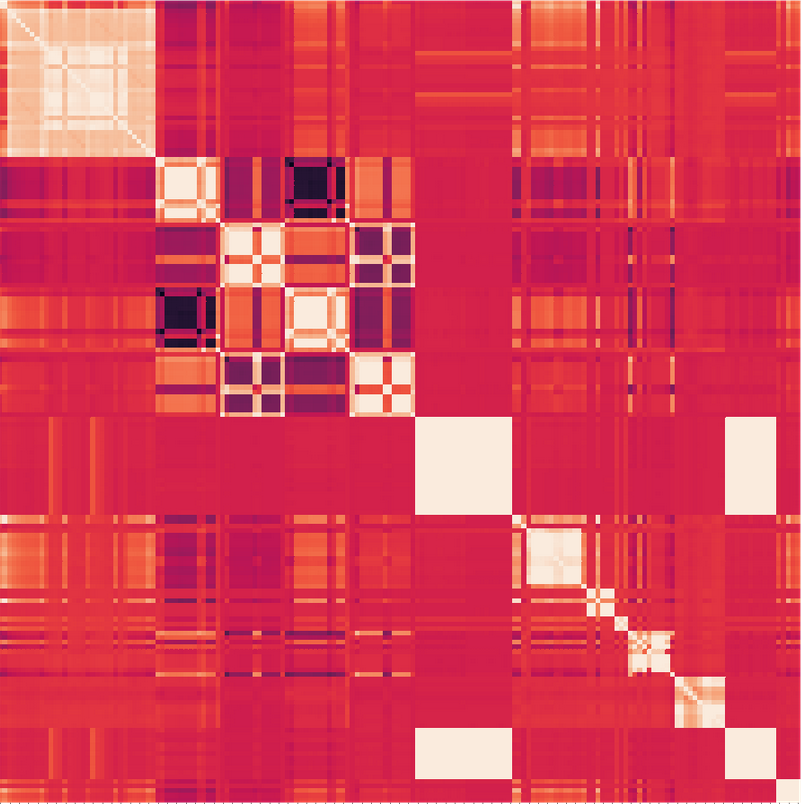
\includegraphics[width=0.5\textwidth]{Correlation_Matric.png}
    \caption{Correlation Matric}
    \label{fig:Correlation Matric}
\end{figure}

\begin{table}[]
\centering
\begin{tabular}{|c|}
\hline  
feature\\
cpu1.usage\\
cpu2.usage\\
...  \\
mem\_cached\\
mem\_buffers\_cache\_free\\
memory.swap\\ 
disk.used.sda1\\
disk.used.sda2\\
...\\
channeltraffic\_in\\
channeltraffic\_in\\
ioutil\_util\_sda\\
ioutil\_util\_sdb\\
ioutil\_util\_sdc\\
ioutil\_util\_sdd\\
...\\
iowait.wait\\
hitratio.port8101\\
hitratio.port8102\\
...\\
\hline 
aggregate.cpi\\
aggregate.diskused\\
aggregated.ioutil\\
aggregate.CPU.max\\
....\\
\hline 
aggregate.all\_machine.cpi\\
aggregate.all\_machine.diskused\\
aggregated.all\_machine.ioutil\\
aggregate.all\_machine.CPU.max\\
\hline 
\end{tabular}
\caption{list of candidate input features from one cache server,We organize the features into groups. The first group is the raw data we directly collected from the caching servers. The second group are the features we construct based on statistics of the metrics of a single machine. The third group are the features we construct based on the statistics of the metrics of the whole group of machines}
\label{my-label}
\end{table}



\subsection{Prediction Model Design}

In this section, we introduce how the architecture we use to predict \dabiaolv of CDN cache group using the data ouput from the feature engineering stage. 

Prior to fitting the data prediction model, we first conduct a pre-training step to fit an encoder that can extract useful and representative embeddings froma  time  series.  The  goals  are  to  ensure  that  (i)  the  learned embedding  provides  useful  features  for  prediction  and  (ii) unusual input can be captured in the embedded space, which will get further propagated to the prediction network in the next step.


lstm encoder-decoder:

prediction networks

\section{Evaluation}
\subsection{Experimental Settings}
Our implementation using the Google machine learning library, Tensorflow, version 1.2.0. We ran our experiments on a physical machine running an Ubuntu 16.04 imag, interl i7, 8 GB memory, and GPU gtx1060.
The data is collected from the daily operation of CDN cache groups
In this section, we illustrate the model performance using \dabiaolv data collected from a cache group in a selected PoP that provide content caching service for several customers. 

In the experiments, 10-fold cross validation is used to eval-
uate the accuracy of predictions. This divides the entire data
set into 10 equal parts.  Prediction is repeated 10 times, each
time keeping one of the 10 parts as test data and the other 9
parts as training data to build the prediction model. Finally,
test results on all the 10 parts are accumulated together to
calculate the average prediction accuracy.

Training procedure We use minibatch stochastic gradient descent (SGD) together with the Adam optimizer [Kingma and Ba, 2014] to train the model. The size of the minibatch is 128. the parameters can be learned by standard back propaga- tion with mean squared error as the objective function:

Loss={}





\subsection{Baseline}
We compare our model with other baseline model which are listed follow:
\begin{enumerate}
  \item VAR Model: a linear model that takes last ouput as the prediction
  \item basic Three layer neural network
  \item Vanilla LSTM Model
  \item LSTM encoder-decoder with multiple-layers perceptions
  \item LSTM encoder-decoder with SVM
\end{enumerate}

To measure the effectiveness of various methods for prediction, we consider three different evaluation metrics. Among them, root mean squared error (RMSE) [Plu- towski et al., 1996] and mean absolute error (MAE) are two scale-dependent measures, and mean absolute percentage error (MAPE) is a scale-dependent measure. Specifically, assuming yt is the target at time t and yt is the predicted value at time t, RMSE is defined as RSME={} and MAE is denoted as MAE={}. When comparing the prediction performance across different datasets, mean absolute percentage error is popular because it measures the prediction deviation proportion in terms of the true values, i.e, MAPE={}.


\subsection{Performance}
\begin{table}[]
\centering
\caption{My caption}
\label{my-label}
\begin{tabular}{lllll}
location & Persistent & LSTM & LSTM encoder-decoder & Our model \\
Shanghai & 10.0       & 9.9  & 8.8                  & 7.7       \\
Shenzhen & 10.0       & 9.9  & 8.8                  & 7.7       \\
Zhejiang & 10.0       & 9.9  & 8.8                  & 7.7      
\end{tabular}
\end{table}

\begin{figure}[h]
    \centering
    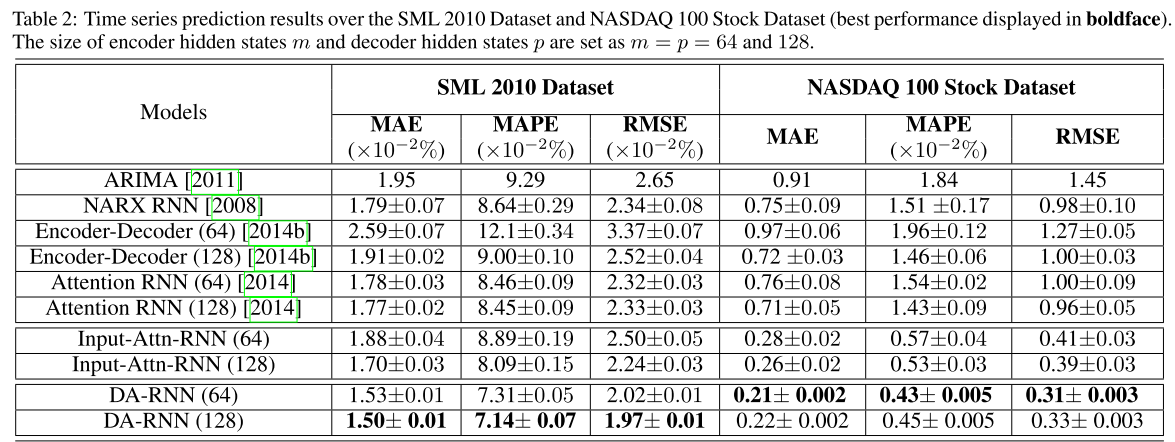
\includegraphics[width=0.5\textwidth]{prediction_results.png}
    \caption{Prediction Results}
    \label{fig:Prediction Results}
\end{figure}

compare four different models in terms of training time and accuracy 

\section{Discussion and Future Work}
As there are hundreds cache group in China. Although our method can be used to train on all kinds of cache group of different architecture, the model for one specific cahce group, a unified models for all kinds of cache groups is required. As qualified rate is an indirect measurement of QoS of clients,collecting data from clients ends will provide useful insights. We also want to develop the online training methods for our models because we observe that the relationship change over time.
\section{Related Work}
When evaluating the's complex system, the evaluation method can fall into three catogory: model-driven method, data-driven method. In model-drvien method, the mathematical model characterizing the inner 
components of a system has to be all known{\Rethinking_CDN}. 

The data characterizing the state of system instead of the analytical model is neceessary. \cite{Jiang2017Pytheas}.\cite{Mao2017NeuralPensieve}.\cite{c}. [From the characteristics of the above methods, the data driven method, which takes the gathered data
as basis and is independent of the object’s prior knowledge, is a more
useful approach for fault prediction and reliability evaluation]l

There are three CDN resarch are (1) long-term network planning, including optimized CDN design that relates to PoP selection and cache deployment, and (2) short-term, run-time cache management, including content replacement and prefetching strategies in the CDN network \cite{Rethinking_CDN}. (3) CDN selection from the client\cite{Jiang2017Pytheas:Exploration-Exploitation} \cite{CFA}. Our research falls in the second catogries. Our performance model can provide a decision basis

deep-learning; RNN; RNN encoder-decoder; LSTM; LSTM time-series application; LSTM with attention; sequence learning with lstm:
Real-Time Prediction of Taxi Demand Using Recurrent Neural Networks

Deep learning has been widely used in performance modeling. 

\section{Conclusion}

In this paper we present a deep learning framwork to evaluate the performance of cache group. This paper shows that it is feasible to apply state-of-the-art Deep learning techniques to model networked systems that provides esimation for its performance. The empirical studies shows that it has outputforms the traditional linear method.
\section*{References}

\bibliographystyle{unsrt}
\bibliography{mendeley}

\end{document}